\pgfplotsset{
  test-axis/.style = {
    legend pos = north east,
    scale only axis
  }
}


\chapter{Исследовательский раздел}


\section{Производительность}
Двумя основными характеристиками, влияющими на производительность, являются время шага симуляции $\Delta t$ и количество моделируемых частиц $N$. Замеры производительности проводятся с использованием одной видеокарты\footnote{Nvidia GeForce GTX 750.}.

\subsection{Допустимое время симуляции}
Зафиксируем частоту кадров при рендеринге каркаса и исследуем зависимость частоты шагов симуляции от количества частиц (рис.~\ref{fig:steps-graph}). Мы можем наблюдать зависимость, близкую к обратной пропорциональности: $\frac{1}{\min\Delta t}\propto \frac{1}{N}$. Отсюда можно сделать вывод, что $\min\Delta t\propto N$.
\begin{figure}[h]
  \centering

  \resizebox{.8\textwidth}{!} {
    \begin{tikzpicture}
      \begin{axis}[
          test-axis,
          ylabel = {Шагов/сек},
          xlabel = {Частиц, тыс},
          ytick = {0, 100, 200, ..., 700},
          xtick = {0, 100, 200, ..., 500},
          xmin = 0,
          xmax = 525,
          domain = 0:700
        ]
        \legend{$\Delta t=5\text{мс}$, $\Delta t=10\text{мс}$}
        \addplot[green, dashed]{200};
        \addplot[red, dashed]{100};
        \addplot[smooth, mark = x] coordinates {
          (25,  660)
          (50,  340)
          (75,  240)
          (100, 180)
          (125, 130)
          (150, 110)
          (175, 100)
          (200, 85)
          (225, 75)
          (250, 70)
          (275, 65)
          (300, 58)
          (350, 45)
          (400, 38)
          (500, 30)
        };
      \end{axis}
    \end{tikzpicture}
  }

  \caption{Зависимость частоты шагов симуляции от количества частиц при 30к/с рендеринге каркаса.}
  \label{fig:steps-graph}
\end{figure}


\subsection{Частота кадров симуляции реального времени}
Исследуем частоту кадров для симуляции, проводящейся в реальном времени, то есть на один шаг симуляции тратится не более $\Delta t$ (рис.~\ref{fig:fps-graph}). Результаты эксперимента позволяют сделать вывод о пропорциональности количества частиц и частоты кадров: $fps\propto N$.

\begin{figure}[h]
  \centering

  \resizebox{.45\textwidth}{!} {
    \begin{tikzpicture}
      \begin{axis}[
          test-axis,
          ylabel = {Частота кадров},
          xlabel = {Частиц, тыс},
          xtick = {110, 120, ..., 170},
          xmin = 105,
          xmax = 175
        ]
        \addplot[smooth, mark = x] coordinates {
          (110, 60)
          (120, 45)
          (130, 35)
          (140, 28)
          (150, 23)
          (160, 17)
          (170, 10)
        };
      \end{axis}
    \end{tikzpicture}
  }%
  \resizebox{.45\textwidth}{!} {
    \begin{tikzpicture}
      \begin{axis}[
        test-axis,
        ylabel = {Частота кадров},
        xlabel = {Частиц, тыс},
        xtick = {50, 60, ..., 90},
        xmin = 45,
        xmax = 95
        ]
        \addplot[smooth, mark = x] coordinates {
          (50, 60)
          (60, 48)
          (70, 32)
          (80, 15)
          (90, 8)
        };
      \end{axis}
    \end{tikzpicture}
  }
  \caption{Зависимость частоты кадров от количества частиц при $\Delta t=10$мс и $\Delta t=5$мс в режиме реального времени.}
  \label{fig:fps-graph}
\end{figure}


\section{Физические явления}
\subsection{Жидкость в условиях нулевой гравитации}
В условиях нулевой гравитации ($\vect g=\vect 0$) жидкость под действием сил поверхностного натяжения стремится принять форму шара (рис.~\ref{fig:zero-gravity}).

\begin{figure}[h]
  \centering
  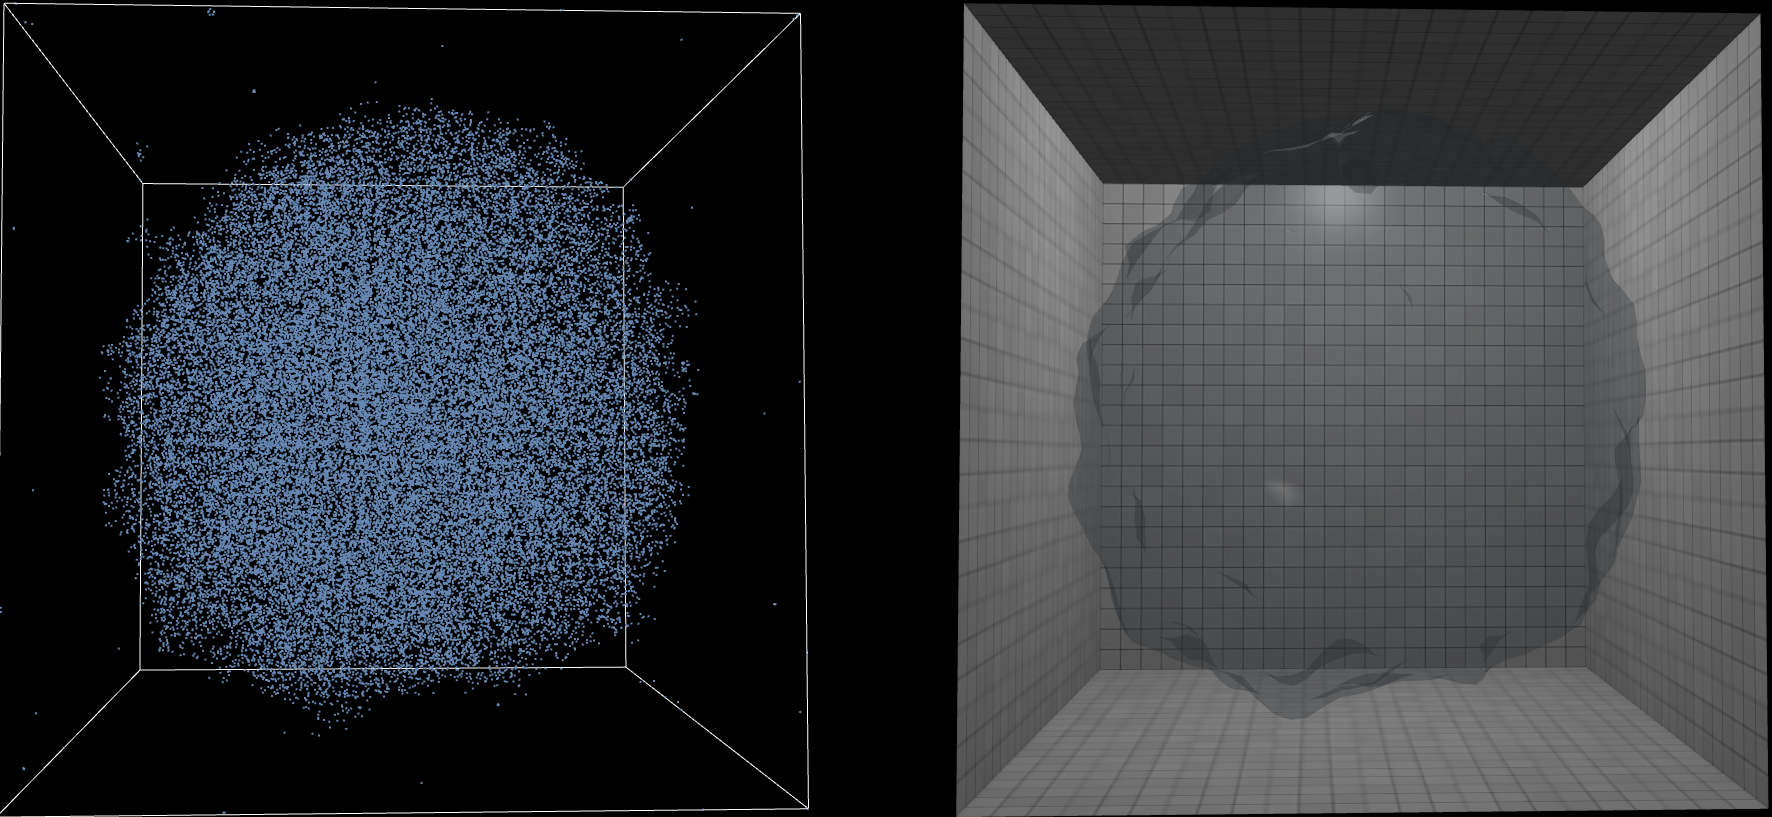
\includegraphics[width=.8\textwidth]{zero-gravity.png}
  \caption{Жидкость в условиях нулевой гравитации.}
  \label{fig:zero-gravity}
\end{figure}
